% !TEX root=../thesis.tex

\chapter{Research Method} % (fold)
% Research questions and method
\label{cha:research_questions_and_method}
In this chapter we will describe the research method used in this 
thesis. We will then describe how the method was used.
\section{Research Methods} % (fold)
\label{sec:research_method}

During the research done in this thesis, we applied the Design Science Research 
Process (DSRP) as the research method. The DSRP is based on 6 steps which are 
presented in the list below. Depending on what the focus of the project is, 
the project can start at almost any of the steps below. \cite{peffers2006design}

\begin{enumerate}
	\item \textbf{Problem identification and motivation} - Defines the problem to be
	researched. 
	\item \textbf{Objectives of a solution} - Infer the goals of the solution.
	\item \textbf{Design and development} - Creates an artifact for the solution.
	\item \textbf{Demonstration} - Demonstrate the created artifact.
	\item \textbf{Evaluation} - Observe and measure how the artifact gives a 
	solution to the problem.
	\item \textbf{Communication} - Communicate the problem along with the artifact.
\end{enumerate}

As Hevner, March, Park, and Ram \cite{von2004design} describes, 
evaluation of a product, created through a sequence of expert activities, 
provides feedback information and a better understanding of the problem in 
order to determine the quality of the product. A process loop which is typically 
iterated a number of times before the final design artifact is generated is created 
by repeating the sequence of expert activities. An example of the process loop 
is demonstrated in \Ref{fig:DSRP}, where one can see the loop as going 
from step 2 (Objectives of a solution) to step 5 (Evaluation) and back.\\

A literature study was performed and workshops were held, as part of the 
method to define the objectives of the solution in step 2. Since the literature study 
reveals what kind of relevant systems that exists and how they fit to the
requirements of the stakeholders, the study helps define the objectives. Focus
groups can be a great way to learn about the work that occurs "between" and 
"around" the solutions \cite{FocusGroupstoStudyWorkPractice}, as focus groups
can have a more relax mood which can lead to more information then for 
instance a prepared questionnaire.

To help answer the research question, a prototype was developed as part of the 
method in the Third step. Developing the prototype helps us understand the 
user and criterias needed for having a system capable of providing stakeholder 
awareness.

Minor pilot studies were performed each week as part of the demonstration and
evaluation in step 4 \& 5. The studies were used as a measurement of the prototype developed
as the method in step 3 against the requirements. Evaluation were then
performed and lead to another execution in the process loop.

\begin{figure}[!htbp]
	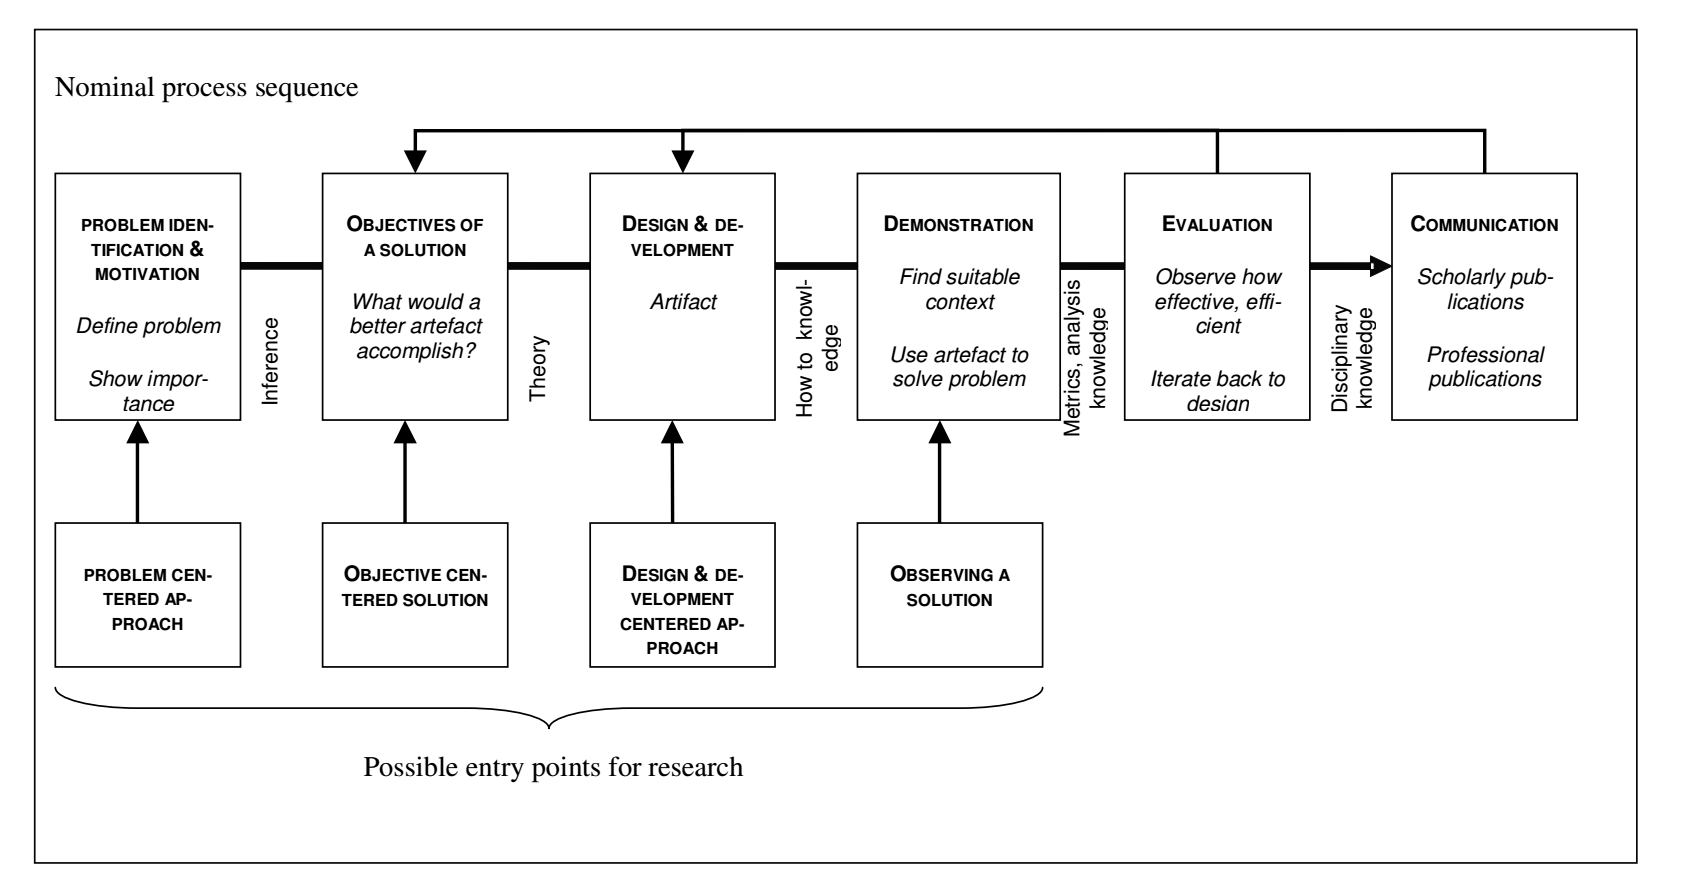
\includegraphics[width=\textwidth,center]{dsrp_modell.png}
	\caption[Design science research process (DSRP) model]{Design research process (DSRP)
	model\cite{peffers2006design}}
	\label{fig:DSRP}
\end{figure}


% section research_method (end)

\section{Project Research} % (fold)
\label{sec:workshops}
In this thesis, the problem was 
identified and motivated prior to the thesis, thus the natural starting 
point of this research was to go into the second stage; objective 
centered. \Ref{fig:DSRP} shows four entry points into a design 
research process; Problem centered-, objective centered-, design \& development-
centered-approach and observing a solution. 

This thesis was an interaction between objectives of a solution, and a study 
of prior art. Examining the state-of-the-art and existing systems is done by 
searching for scientific articles and commercial systems which contribute 
towards the goal of the thesis, and has been performed as a part of the 
background study. We are able to detect the holes in the available 
functionality, by describing and categorizing the systems found in the case 
study. As part of defining the objectives of the solution, we compared the 
provided functionality by the systems against the stakeholders and their 
requirements.\\

Two workshops were held as part of defining the goals of the solution and the 
prototype for step 2, define the needs of the stakeholders, and as part of the 
requirements elicitation. Several stakeholders were participating in these
workshops helped define the direction of the process. By using a focus group 
consisting of stakeholders, we were able to help define specifications for the 
system and the domain. 
%We are also guaranteed the if the specification is implemented as a machine which is subsequently connected to the environment, then the requirements will be satisfied \cite{zave1997four}. 


By putting together a focus group, one can utilize stakeholders to define the
objectives of a solution. As Nielsen \cite{FocusGroupstoStudyWorkPractice} 
says, focus groups can be a great way to learn about the work that occurs 
"between" and "around" the solutions. Focus groups have the advantage of allowing more natural interactions between people than interviews. One is often able to bring out users spontaneous reactions and ideas \cite{nielsen1997use}, 
by bringing together several users. To ensure that these focus groups stays 
focused during the entire workshops, the moderator have to make sure the 
groups discusses a pre planned set of issues and set goals for the kind of 
information to be gathered. The use of focus groups within requirements 
engineering have become more popular, because of their claim to greatly 
accelerate the development of requirements \cite{goguen1993techniques}. \\

As part of the iterative process loop, a pilot study with the supervisors was 
held each week. During these meetings the current status of both the case 
study and development of the prototype was demonstrated. The demonstrations 
were performed as the observational evaluation method case study, where the 
artifact is studied in depth in business environment \cite{von2004design}. The 
evaluation involves comparing the objectives of the solution to actual 
observed results from use of the artifact in the demonstration 
\cite{peffers2006design}, and was performed as a comparison of the prototype's 
functionality with the solution objectives defined in step 2. \\

The final step of the process, communication of the results are done through this thesis.

% section workshops (end)

% chapter research_questions_and_method (end)

